\openingarticle
\def\ppages{\pagerange{asapa:firstpage}{asapa:lastpage}}
\def\shorttitle{A review of the ASAPA Conference from the 1st -3rd July 2015}
\def\maintitle{Taking stock of archaeological thought, method and practice in southern Africa. A review of the ASAPA Conference from the \nth{1}--\nth{3} July 2015}
\def\shortauthor{Jacqueline Jordaan}
\def\authormail{jacquelinejordaan@outlook.com}
\def\affiliation{University of Manitoba}
\def\thanknote{\footnote{Thank you to the members of the Local Organising Committee, and the various funders and supporters of the conference: ASAPA, University of Zimbabwe, Confucius Institute, Republique Francaise, The National Museums and Monuments of Zimbabwe, The United Nations Educational, Scientific and Cultural Organization, The Wenner- Gren Foundation.	Acknowledgements also need to be given to the Palaeontological Scientific Trust (PAST) and its Scatterlings of Africa programmes for the allocation of funds for my attendance of the conference.  Lastly, thanks are given to G. Jordaan, and T. Forssman, and subsequent reviewers, for their comments on this document.}}
%--------------------------------------------------------------
\mychapter{\maintitle}
\begin{center}
	{\Large\scshape\shortauthor \thanknote}\\[1em]
	\email \\
	\affiliation
\end{center}
\vspace{3em}
\midarticle
%--------------------------------------------------------------
\label{asapa:firstpage}


	
	\lettrine[nindent=0em,lines=3]{T}{he} biennial conference of the Association of Southern African Professional Archaeologists (ASAPA) was hosted in Zimbabwe, at the University of Zimbabwe (Harare) . The conference theme, “\textit{Towards an interdisciplinary framework for southern African archaeology: Taking stock of archaeological thought, methods and practice}”, was appropriate, albeit poorly realised at the conference.
	 
	The proceedings were opened by plenary talks given by Innocent Pikirayi (University of Pretoria), Judith Sealy (University of Cape Town), Gilbert Pwiti (University of Zimbabwe), and Simon Hall (University of Cape Town). Each speaker reflected on the background and development of archaeology in the region, and noted key ideas for the future development of the discipline. Pikirayi discussed a key issue in African archaeology, that of the need to decolonise the practice across the continent, in his speech ‘\textit{Breaking barriers and decolonising practice: Towards an African Archaeology of the Future}’. A talk was given by Sealy on ‘Archaeological science in Southern Africa archaeology today: contributions and challenges’ in which an appeal was made for researchers to address the ‘grand challenges’ in archaeology. She asked researchers to consider ‘what are the key questions we, as a region, are trying to answer, and how best could we bring the key questions and scientific techniques together?’ The talk resonated with much of the audience and left an impression, with multiple references from other conference presenters. The next talk was given by Prof. Pwiti on ‘\textit{Archaeological heritage management in southern Africa}’. He discussed the different perspectives encountered within heritage management in the region, and noted how these varying perspectives complicated as well as contributed to the practice of heritage managers locally. Presenting on the topic of the recent past, and it’s handling in a dynamic political present was Prof. Hall’s speech ‘\textit{The Go-Between? Historical Archaeology in Southern Africa}’. He called for researchers to be aware of the contemporary context of their research, and to act responsibly in light of this awareness. In his speech, Hall referenced the recent removal of the controversial Cecil John Rhodes Statue from the grounds of University of Cape Town as an example.  Rather than using heritage as a space for discussion, to de-nature politics and bolster unity as a nation, it simply became a symbol of racism. Hall’s message was ironically held true just days after the conference, when an opinion piece was published in the ‘The Herald’ (Zimbabwe’s largest daily newspaper). The piece titled ‘\textit{Africa must rid itself of imperialistic symbols}’ cited both Prof. Pikirayi and Prof. Hall’s remarks on the Rhodes statue debate (Tsiko 2015)\texttt{}\footnote{Tsiko, S. 2015. ‘Zimbabwe: Africa Must Rid Itself of Imperialistic Symbols’, The Herald [online allafrica], 9 July, available \href{http://allafrica.com/stories/201507090355.html}{here}.}. These presentations, and their after-effects, remind us that archaeological knowledge is not isolated from a present socio-political discourse. 
	
\begin{figure}
			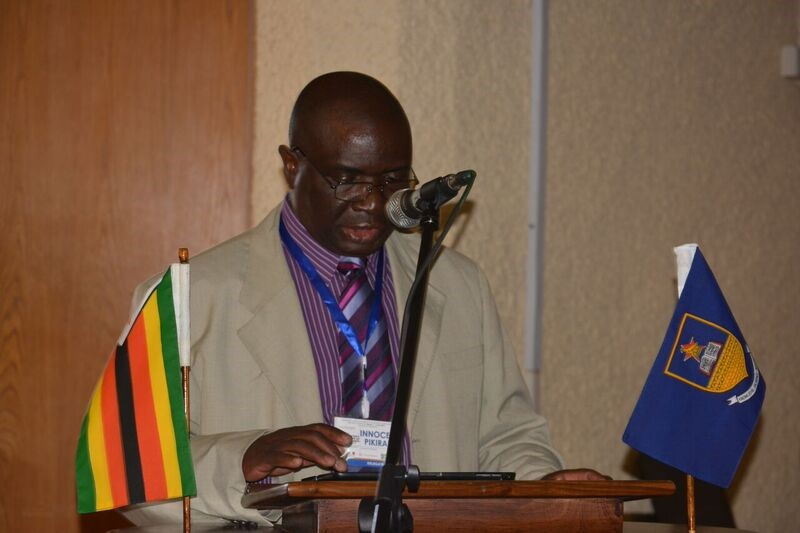
\includegraphics[width=\linewidth]{figures/asapa_01}%<<-- the relative-path of the figure --> it is stored in the folder "figures" and its filename is "testfigure"
			\caption{Prof. Pikirayi presenting his plenary (photo courtesy of Carlton Rambanapasi).}
			\label{asapa_01} %best is to use the name of the file
		\end{figure}
	
	Following the opening presentations, a range of sessions ensued. The sessions held at the conference were under the following topics: ‘Early, Middle and Late Stone Age’, ‘Archaeo-Mining’, ‘Archaeo-Metallurgy’, ‘Heritage, Archaeology’ and ‘Education’, ‘Hunter Gather and Farmer Interactions’, ‘Spatial Archaeology’, ‘Farmer Communities Archaeology’, ‘Climate Variability and Archaeology’, ‘Material Culture and Identities’, ‘Rock-Art’, ‘Historical Archaeology’, ‘Ethnoarchaeology’, ‘Conservation’, and ‘Archaeozoology’\footnote{For a more detailed list of conference sessions and presenter titles, follow this \href{http://www.asapa2015.uz.ac.zw/index.php/conference/programme}{link}, also the conference proceedings are set to be published the following year.}. The sessions reflected the diverse interests of practitioners in the region. However, an intense focus was placed on heritage with five sessions dedicated to the various aspects of this topic. Re-enforcing the bearing of the plenary speeches, heritage and what that construes has become ubiquitous in discourse between archaeologists, as well as other stakeholders, in the region.
	
	The conference also encouraged platforms for student presentations and networking\footnote{For further details regarding SAASC, and the student blitz session, please visit this \href{http://saasc.co.za/index.php/2015/07/21/asapa-2015-student-blitz-session/}{link}.}, and rewarded student excellence in the form of the Ray Inkskeep awards. An ASAPA conference first was the ‘Student Blitz Session’ chaired by the Southern African Archaeology Student Council (SAASC). The session was a platform for a diverse range of topics presented by archaeology students from all over southern Africa. Each presenter had five minutes to present their topic. The topics ranged from presentations on ‘The application of methods’, ‘The role of various media platforms in public archaeology and research’ and ‘Research projects and agendas’. This session provided a platform for students to share their thoughts and research, and provided a glimpse of the diverse avenues which students of southern African archaeology traverse. The following evening students were able to socialise at the student quiz night. The night was an evening of roaring laughter and fierce competition. It provided a much needed opportunity for students from across southern Africa to meet in a casual setting. 
		
	\begin{figure}
		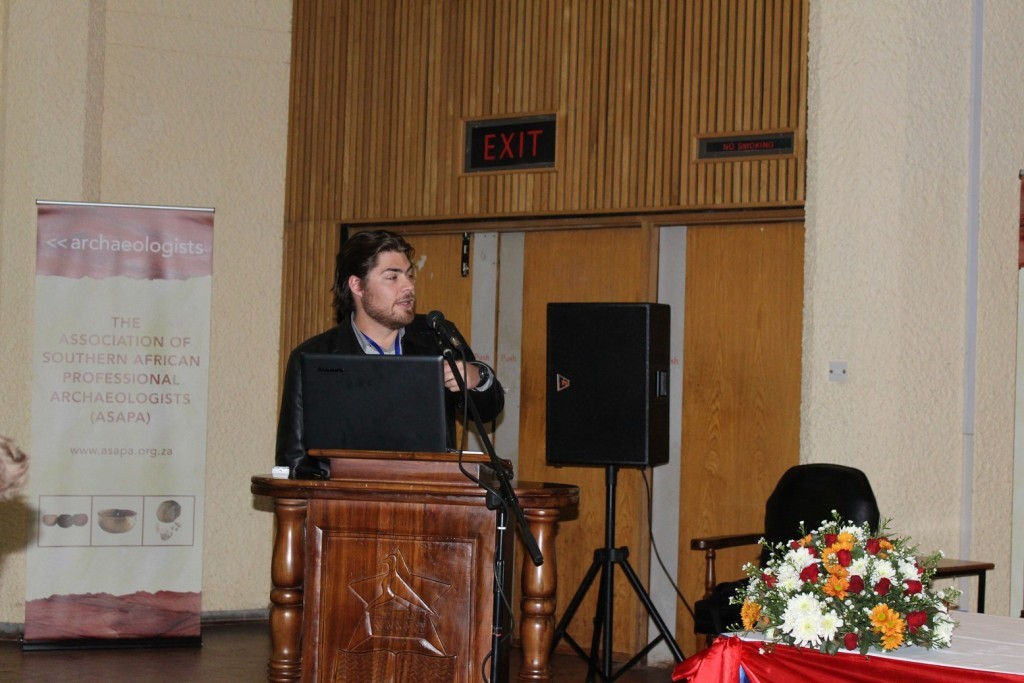
\includegraphics[width=\linewidth]{figures/asapa_02}%<<-- the relative-path of the figure --> it is stored in the folder "figures" and its filename is "testfigure"
		\caption{David Witelson presenting in the 'Student Blitz session' (photo courtesy of Lu-Marie Fraser).}
		\label{asapa_02} %best is to use the name of the file
	\end{figure}
	
	\begin{figure}
		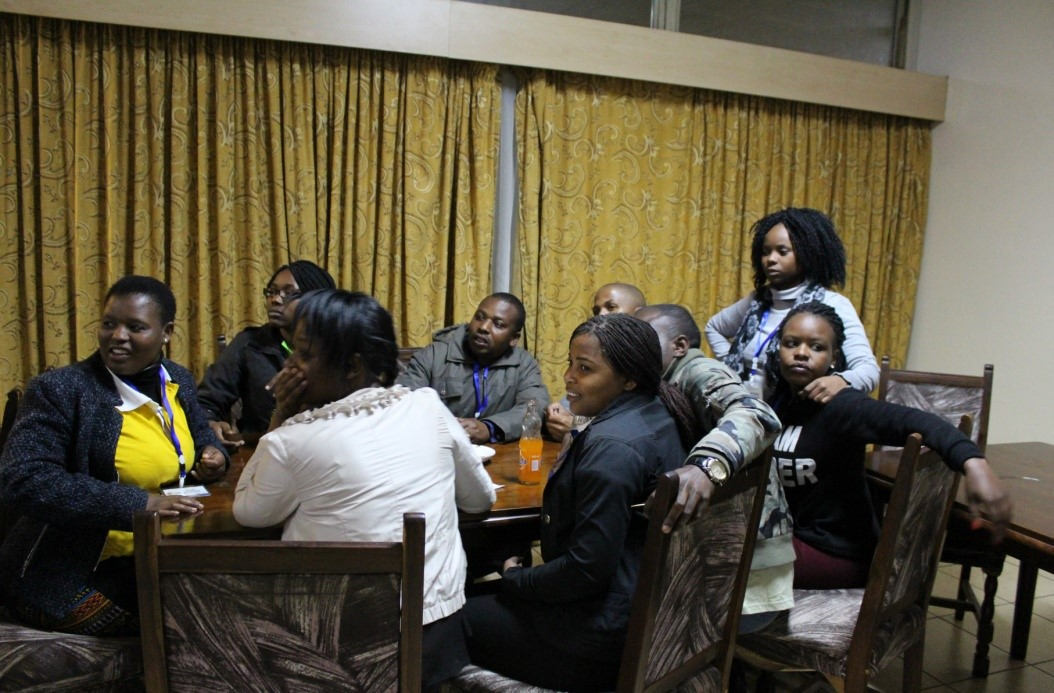
\includegraphics[width=\linewidth]{figures/asapa_03}%<<-- the relative-path of the figure --> it is stored in the folder "figures" and its filename is "testfigure"
		\caption{A quiz team at SAASC student night (photo courtesy of Lu-Marie Fraser).}
		\label{asapa_03} %best is to use the name of the file
	\end{figure}
	
	Continuing along the theme of student interest, the Ray Inkskeep Award was presented this year at the conference. In honour of the late Prof. Inkskeep, an important figure in the development of archaeology in the southern African region, two awards were given. The first award for best student oral presentation was given to E. Grody, for the presentation ‘\textit{Of Buffalo and Butchers: Coupling traditional procurement studies with taphonomic analyses to explore wild processing patterns at two Early Iron Age Sites in the Kruger National Park}’, and the runner-up award was given to N. Mokoena, for the presentation ‘\textit{What is your heritage? Communities’ Perceptions on Heritage and Rock Art: The Case of Rural South Africa}’.  Both presented novel and outstanding papers, and were fair winners of the prize. 
				
	To end with a note on the conference's theme in mind, the full stock and diversity of archaeological thought, methods and practice in southern African archaeology was not exhibited at the conference, because a majority of southern African archaeology practitioners did not attend the conference.  This is testified by the fact that the number of delegates, those with ASAPA membership, was so low that the bi-annual general meeting of ASAPA members could not be held. In of itself this has repercussions for the broader discipline in the region, as the general meeting is a time for bi-annual review and election of new council members. How do we expect the discipline to grow in southern Africa if we don’t make the effort to meet and discuss our objectives and research? There are assuredly reasons for this low attendance of the conference; however, is it not our responsibility to make an effort for the betterment of the discipline? 
	
		

\label{asapa:lastpage}
\closingarticle
